\documentclass[40pt,a4paper,UTF8,twocolumn]{ctexart}%设置字号,编码,排版为2栏
\usepackage{amsmath}
\usepackage{graphicx}

\usepackage{float}

%输入带圈数字  eg:\textcircled{1}
\usepackage{fontspec,xunicode-addon}

%代码显示的包
\usepackage{listings}
\usepackage{xcolor}

%打出空心字母
\usepackage{amsfonts,amssymb}

%整体加粗
\usepackage{bm}

%公式按照章节标号
\numberwithin{equation}{section}

%长等号
\usepackage{extpfeil}

%列举
\usepackage{enumerate}

%注释用
\usepackage{comment}

%自定义标题格式
\usepackage{titlesec}



%----------------------------------------------
%配置代码显示格式-掌握minted之前的替代品
%----------------------------------------------
\definecolor{codegreen}{rgb}{0,0.6,0}
\definecolor{codegray}{rgb}{0.5,0.5,0.5}
\definecolor{codepurple}{rgb}{0.58,0,0.82}
\definecolor{backcolour}{rgb}{0.95,0.95,0.92}

\lstdefinestyle{mystyle}{
	backgroundcolor=\color{backcolour},   
	commentstyle=\color{codegreen},
	keywordstyle=\color{magenta},
	numberstyle=\tiny\color{codegray},
	stringstyle=\color{codepurple},
	basicstyle=\ttfamily\footnotesize,
	breakatwhitespace=false,         
	breaklines=true,                 
	captionpos=b,                    
	keepspaces=true,                 
	numbers=left,                    
	numbersep=5pt,                  
	showspaces=false,                
	showstringspaces=false,
	showtabs=false,                  
	tabsize=2
}

\lstset{style=mystyle}

% article、report或book通常会将\section{}标题居中或者按照一定的缩进对齐
% 重新定义了\section的显示样式,使其左对齐。
\titleformat{\section}
  {\normalfont\Large\bfseries}{\thesection}{1em}{}

\title{Motion planning homework 5}
\author{Student name: Francisrk}
\date{Due date: February 20th, 2024}


%-----------------------------------------------------------------------------------


\begin{document}	
\maketitle   %控制序列,能将在导言区中定义的标题、作者、日期按照预定的格式展现出来。

% %这个\twocolumn[]应该是在[]范围内的使用单栏排版。
% \twocolumn[
% \begin{@twocolumnfalse}
% \maketitle   %控制序列,能将在导言区中定义的标题、作者、日期按照预定的格式展现出来。
% \begin{abstract}

% 这里是中文摘要。我国飞速发展的企业信息管理技术,已经发展成为了企业进行规范化管理、提高效益的有效途径之一,
% 在加强企业人力资源的管理、减少企业经营运行的成本、增强企业的竞争力等多个方面起着重要作用。


% \textbf{关键词:}这里是关键词。

% %\textbf{Abstract}
% Here is english abstract.
% China's rapid development of enterprise information management technology has developed into 
% an effective way for enterprises to standardize management and improve efficiency, 
% in strengthening the management of human resources, reduce the cost of enterprise operation, 
% enhance the competitiveness of enterprises and other aspects play an important role. 

% \textbf{Keyword:}Keyword、Management Information System、Enterprise Resource Planning、 
% Business Operation Simulation

% \end{abstract}
% \end{@twocolumnfalse}
% ]

% \clearpage  % 第1部分双栏结束后换新页。

\section{第1题}


\subsection{题目}

\begin{figure}[H]
    \centering
    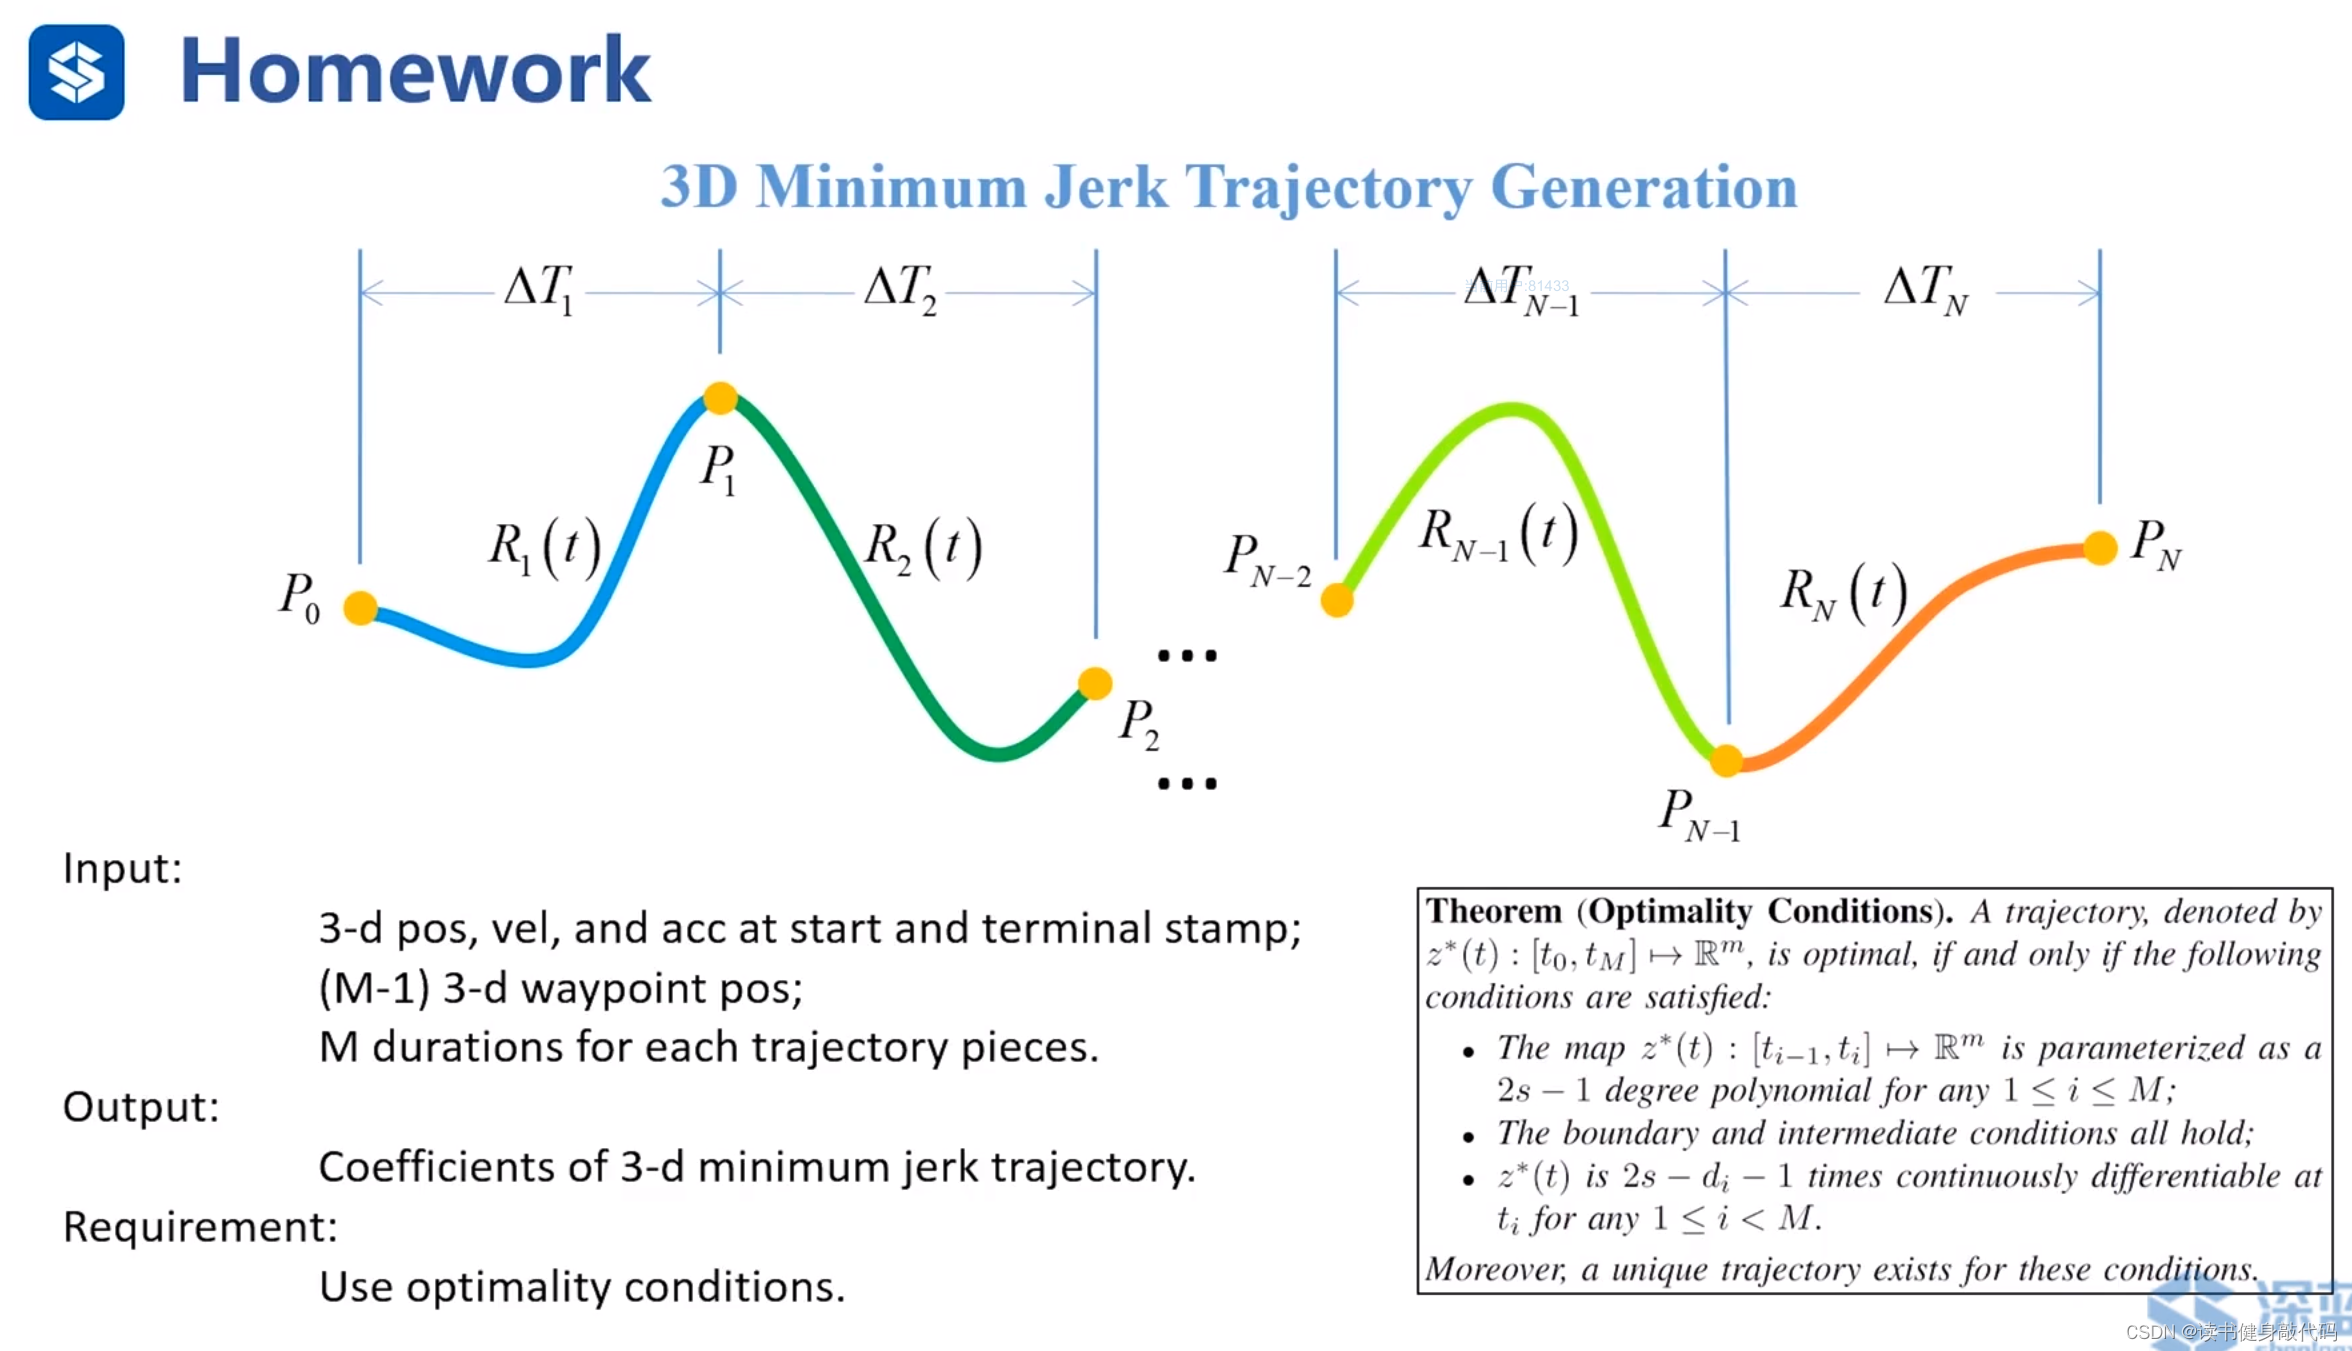
\includegraphics[width=3.0in]{ch5_1.png} 
    \caption{题目描述}
    \label{fig1} % 这里设置标签
\end{figure}

如图\ref{fig1}所示,要求写一个Minimum Jerk的trajectory generation的程序:
\begin{enumerate}
    \item \textbf{输入}
        \begin{enumerate}
            \item start和goal的$(p,v,a)$和时间
            \item $(M-1)$个中间需要经过的的3-d waypoint
            \item 每个segment的time duration
        \end{enumerate}
    \item \textbf{输出}
    
         3\-D的最小化jerk轨迹的solution的系数。(由最优性条件可得,minimum jerk,3阶导数,$s=3$;
         $z^{(d_i-1)}=p=z^{(0)}$,则$d_i=1$,解一个BIVP,则solution是一个$2s-1=5$次多项式)。
    \item \textbf{要求}

        使用最优性条件。
\end{enumerate}

\subsection{求解}
    首先对问题进行分析,参考这里optimality condition的原文\cite{ref1},
    该文章提出一种框架,用于满足几何约束和自定义动态约束的多旋翼的轨迹生成。首先对文章的contribution进行总结:
    
    \begin{enumerate}
        \item 提出并证明最优性条件。
        \item 设计一个能满足复杂约束且为线性复杂度的轨迹类MINCO。
        \item 提出了具有约束消除和约束转换的traj generation框架。
        \item 实验证明了所以出的方法的效率,最优性,鲁棒性和泛化性。
    \end{enumerate}
    具体来说,该文章基于微分平坦特性,提出最优性条件,基于最优性条件,提出一种解决无约束条件下的BIVP的方法,
    该方法能够在线性时间复杂度内完成BIVP的求解。本章作业内容就是使用该方法构建线性方程组
    \begin{equation}
        \bm{Mc}=\bm{b}
        \label{eq1.1} % 这里设置标签
    \end{equation}
    通过求解式(\ref{eq1.1})完成BIVP的求解,而式(\ref{eq1.1})的求解过程是线性时间复杂度的,该方法极大提高了BIVP问题的求解效率。

    针对复杂的带约束的BVP的求解,核心思想是使用不同的方法来消除约束,并降低优化问题的维度,摘要中提及了以下方法用于消除约束:
    \begin{enumerate}
        \item     在多规划约束下对表示进行时空变形。
        \item     使用平滑映射以一种轻量级方式消除几何约束。
        \item    将密集约束评估与稀疏参数化解耦,以及平坦映射的反向微分,支持了多种状态-输入约束。
    \end{enumerate}


    接下来进行具体问题求解。
根据图\ref{fig1}最优性条件,优化jerk,即$z^{(s)}(t)=j(t)$,则$s=3$,中间状态约束只给出waypoints的位置($p$)约束,所以
\begin{gather} %将两个公式放在一起,使用gather
    \bar{z}=z^{(d_i-1)}=z^{(0)} \\
    d_i=1
\end{gather}

所给约束包含边界约束和中间状态约束,分别为\cite{ref1}中的式(18c)(18d):
\begin{figure}[H]
    \centering
    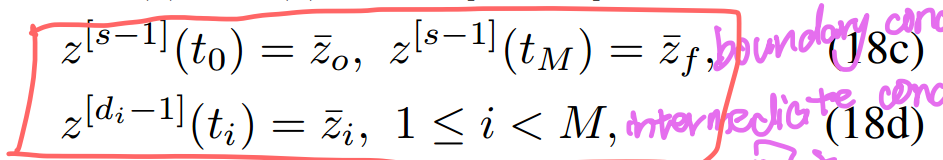
\includegraphics[width=3.0in]{ch5_2.png} 
    \caption{\cite{ref1}的边界约束和中间状态约束}
    \label{fig2} % 这里设置标签
\end{figure}

由optimality condition可得,BIVP的最优平坦输出为$2s-1=5$次多项式,被表示为
\begin{align}
    z^*(t) = c_0+c_1t+c_2t^2+c_3t^3+c_4t^4+c_5t^5 \label{eq1.4}
\end{align}
由optimality condition最后一条可得:
\begin{equation}
    \bar{d_i}=2s-d_i=5    
\end{equation}
$z^*(t)$是$\bar{d_i}-1=5-1=4$阶连续可导的,即其4阶导数存在且连续,其$0-4$阶导数分别为如式(\ref{eq1.6})所示
\begin{equation}
\left\{
    \begin{array}{l}
        z^{(0)}(t)=c_0+c_1t+c_2t^2+c_3t^3+c_4t^4+c_5t^5\\
        z^{(1)}(t)=c_1+2c_2t+3c_3t^2+4c_4t^3+5c_5t^4\\
        z^{(2)}(t)=2c_2+6c_3t+12c_4t^2+20c_5t^3\\
        z^{(3)}(t)=6c_3+24c_4t+60c_5t^2\\
        z^{(4)}(t)=24c_4+120c_5t\\
    \end{array}
\right.
\label{eq1.6} % 这里设置标签
\end{equation}

关于boundary condition。

\textbf{初始条件initial boundary condition}
有$t=0$,且$p_0,v_0,a_0$已知,且有
\begin{gather}
    z^{(0)}(0)=c_0 \label{eq1.7} \\
    z^{(1)}(0)=c_1 \label{eq1.8}\\
    z^{(2)}(0)=c_2 \label{eq1.9}\\ 
    \notag % 这里设置标签
\end{gather}
式(\ref{eq1.7})$-$(\ref{eq1.9})分别为initial $p_0,v_0,a_0$,由于$z^*(t)$的形式由(\ref{eq1.4})给出,
所以只要求出所有系数$c_i,i\in(1,2,3,4,5)$,即为求出optimal flat output $z^*(t)$。

将式式(\ref{eq1.7})$-$(\ref{eq1.9})整理为矩阵形式:
\begin{align}
    \begin{bmatrix}
        1&0&0&0&0&0 \\
        0&1&0&0&0&0 \\
        0&0&2&0&0&0 \\
        0&0&0&0&0&0 \\
        0&0&0&0&0&0 \\
        0&0&0&0&0&0
    \end{bmatrix}
    \begin{bmatrix}
        c_0 \\ c_1 \\ c_2 \\ c_3 \\ c_4 \\ c_5 \\
    \end{bmatrix}
    =
    \begin{bmatrix}
        p_0\\v_0\\a_0 \\0\\0\\0
    \end{bmatrix}
\end{align}
进一步整理为
\begin{align}
    \begin{bmatrix}
        1&0&0&0&0&0 \\
        0&1&0&0&0&0 \\
        0&0&2&0&0&0 \\
        0&0&0&0&0&0 \\
        0&0&0&0&0&0 \\
        0&0&0&0&0&0
    \end{bmatrix}
    \begin{bmatrix}
        c_{0x}^0&c_{0y}^0&c_{0z}^0 \\
        c_{1x}^0&c_{1y}^0&c_{1z}^0 \\
        c_{2x}^0&c_{2y}^0&c_{2z}^0 \\
        c_{3x}^0&c_{3y}^0&c_{3z}^0 \\
        c_{4x}^0&c_{4y}^0&c_{4z}^0 \\
        c_{5x}^0&c_{5y}^0&c_{5z}^0 \\
    \end{bmatrix}
    = \notag \\
    \begin{bmatrix}
        p_{x}^0 &p_{y}^0 &p_{z}^0\\ 
        v_{x}^0 &v_{y}^0 &v_{z}^0\\
        a_{x}^0 &a_{y}^0 &a_{z}^0\\
        0&0&0 \\
        0&0&0 \\
        0&0&0
    \end{bmatrix}
    \label{eq1.11}
\end{align}
其中$c_{1x}^0$表示系数$c_1$在$0$时刻的$x$方向的分量,$p_{x}^0$表示为0时刻需要经过的waypoint的$p$的x方向分量,
其他以此类推。

约束均以式(\ref{eq1.11})的形式进行表示,需要构造的式(\ref{eq1.1})即为(\ref{eq1.11})的形式,其中
\begin{equation}
    \bm{F}_0=
    \begin{bmatrix}
        1&0&0&0&0&0 \\
        0&1&0&0&0&0 \\
        0&0&2&0&0&0 \\
        0&0&0&0&0&0 \\
        0&0&0&0&0&0 \\
        0&0&0&0&0&0
    \end{bmatrix}
\end{equation}

$\bm{E_0}=\bm{0},\bm{F_{M}}=\bm{0}$稍后讲解。

\textbf{终止条件terminal boundary condition}
有$t=t_M$,$p_M,v_M,a_M$已知,带入式(\ref{eq1.6})整理可得
\begin{align}
    \begin{bmatrix}
        1&t_M&t_M^2&t_M^3&t_M^4&t_M^5 \\
        1&t_M&t_M^2&t_M^3&t_M^4&t_M^5 \\
        0&1&2t_M&3t_M^2&4t_M^3&5t_M^4 \\
        0&0&2&6t_M&12t_M^2&20t_M^3 \\
        0&0&0&6&24t_M&60t_M^2 \\
        0&0&0&0&24&120t_M
    \end{bmatrix} \cdot \notag \\
    \begin{bmatrix}
        c_{0x}^{t_M}&c_{0y}^{t_M}&c_{0z}^{t_M} \\
        c_{1x}^{t_M}&c_{1y}^{t_M}&c_{1z}^{t_M} \\
        c_{2x}^{t_M}&c_{2y}^{t_M}&c_{2z}^{t_M} \\
        c_{3x}^{t_M}&c_{3y}^{t_M}&c_{3z}^{t_M} \\
        c_{4x}^{t_M}&c_{4y}^{t_M}&c_{4z}^{t_M} \\
        c_{5x}^{t_M}&c_{5y}^{t_M}&c_{5z}^{t_M} 
    \end{bmatrix}
    = 
    \begin{bmatrix}
        p_{x}^{t_M} &p_{y}^{t_M} &p_{0z}^{t_M}\\ 
        v_{x}^{t_M} &v_{y}^{t_M} &v_{0z}^{t_M}\\ 
        a_{x}^{t_M} &a_{y}^{t_M} &a_{0z}^{t_M}\\ 
        0&0&0 \\
        0&0&0 \\
        0&0&0
    \end{bmatrix}
\end{align}
其中
\begin{equation}
    \bm E_M=
    \begin{bmatrix}
        1&t_M&t_M^2&t_M^3&t_M^4&t_M^5 \\
        1&t_M&t_M^2&t_M^3&t_M^4&t_M^5 \\
        0&1&2t_M&3t_M^2&4t_M^3&5t_M^4 \\
        0&0&2&6t_M&12t_M^2&20t_M^3 \\
        0&0&0&6&24t_M&60t_M^2 \\
        0&0&0&0&24&120t_M
    \end{bmatrix}
\end{equation}


针对\textbf{中间状态约束intermediate condition}由optimality condition第4条可知,$z^*(t)$4阶连续可导,
且中间状态约束仅有$p$,即只需要经过某些指定的waypoint,并不指定经过时的velocity,acceleration,jerk,snap,
所以由式(\ref{eq1.6})和intermediate condition可分别构建中间状态的线性方程组,
我们以$\bm{C_1},\bm{C_2}$分别代表第1和第2段piece的optimal flat output,设$\bm_{C_1},\bm_{C_2}$段分配的时间分别为$t_1,t_2$
\begin{enumerate}
    \item $\bm{C_1}$轨迹终点为指定的$p^{t_1}$
    带入式(\ref{eq1.6})得
    \begin{equation}
        c_0+c_1t_1+c_2t_1^2+c_3t_1^3+c_4t_1^4+c_5t_1^5=p^{t_1}
    \end{equation}
    其中$\bm p^{t_1}$为$\bm{C_1}$末时刻经过的位置,整理得
    \begin{equation}
        \left\{
            \begin{array}{l}
                \bm E_{1\_1}=
                \begin{bmatrix}
                    1&t_1&t_1^2&t_1^3&t_1^4&t_1^5
                \end{bmatrix}\\
                \bm F_{1\_1}=
                \begin{bmatrix}
                    0&0&0&0&0&0
                \end{bmatrix}\\
                \bm b_{1\_1} = 
                \begin{bmatrix}
                    p^{t_1}_x & p^{t_1}_y & p^{t_1}_z
                \end{bmatrix}\\
            \end{array}
        \right.
        \label{eq1.6} % 这里设置标签
    \end{equation}
    其中$E_{1\_1}$前后两个1分别表示第1个中间状态约束的第1项。
    \item $z^*(t)$的0阶导数存在且连续,即$\bm{C_1}$轨迹终点为$\bm{C_1}$轨迹起点,
    带入式(\ref{eq1.6})得
    \begin{equation}
        c_0+c_1t_1+c_2t_1^2+c_3t_1^3+c_4t_1^4+c_5t_1^5=p^{t_2}
        \label{eq1.17}
    \end{equation}
    其中$p^{t_2}$为$\bm{C_2}$的起始时刻经过的位置,由于每个segment都是使用的相对时间,所以在$\bm{C_2}$的起始时刻,$t=0$,
    带入式(\ref{eq1.6})得$p^{t_2}=c_0$,带入式(\ref{eq1.17}),移项整理得
        \begin{equation}
            \left\{
                \begin{array}{l}
                    E_{1\_2}=
                    \begin{bmatrix}
                        1&t_1&t_1^2&t_1^3&t_1^4&t_1^5
                    \end{bmatrix}\\
                    F_{1\_2}=
                    \begin{bmatrix}
                        -1&0&0&0&0&0
                    \end{bmatrix}\\
                    b_{1\_2} = 
                    \begin{bmatrix}
                       0 & 0 & 0
                    \end{bmatrix}\\
                \end{array}
            \right.
            \label{eq1.6} % 这里设置标签
        \end{equation}
    接下来具体解释式(\ref{eq1.1})的具体形式,针对每个中间状态约束而言,式(\ref{eq1.1})的形式为
    \begin{equation}
        \begin{pmatrix}
            \bm E_i & \bm F_i
        \end{pmatrix}
        \begin{pmatrix}
            \bm c_i \\ \bm c_{i+1}
        \end{pmatrix}
        =
        \begin{pmatrix}
            \bm D_i \\ \bm 0_{\bar{d_i}\times m}
        \end{pmatrix}
    \end{equation}
    其中$\bm E_i$在这个上下文中表示$\bm C_1$段的约束,$\bm F_i$表示$\bm C_2$段的约束,
    $\bm c_i, \bm c_{i+1}$分别表示$\bm C_1,\bm C_2$段piece的optimal flat output的系数。
    
    按照该思路依次推导剩余的velocity,acceleration,jerk,snap连续时的中间状态约束。
    \item 速度连续,$\bm v^{t_2}=\bm c_1$
    \begin{equation}
        \bm c_1+2\bm c_2t_1+3\bm c_3t_1^2+4\bm c_4t_1^3+5c_5t_1^4=\bm c_1
    \end{equation}
    整理得
    \begin{equation}
        \left\{
            \begin{array}{l}
                \bm E_{1\_3}=
                \begin{bmatrix}
                    0&1&2t_1&3t_1^2&4t_1^3&5t_1^4
                \end{bmatrix}\\
                \bm F_{1\_3}=
                \begin{bmatrix}
                    0&-1&0&0&0&0
                \end{bmatrix}\\
                \bm b_{1\_3} = 
                \begin{bmatrix}
                    0 & 0 & 0
                \end{bmatrix}\\
            \end{array}
        \right.
        \label{eq1.6} % 这里设置标签
    \end{equation}

    \item 加速度连续,$\bm a^{t_2}= 2\bm c_2$
    \begin{equation}
        2\bm c_2+6 \bm c_3t_1+12 \bm c_4t_1^2+20 \bm c_5t_1^3=\bm c_2
    \end{equation}
    整理得
    \begin{equation}
        \left\{
            \begin{array}{l}
                \bm E_{1\_4}=
                \begin{bmatrix}
                    0&0&2&6t_1&12t_1^2&20t_1^3
                \end{bmatrix}\\
                \bm F_{1\_4}=
                \begin{bmatrix}
                    0&0&-2&0&0&0
                \end{bmatrix}\\
                \bm b_{1\_4} = 
                \begin{bmatrix}
                    0 & 0 & 0
                \end{bmatrix}\\
            \end{array}
        \right.
        \label{eq1.6} % 这里设置标签
    \end{equation}
    % z^{(2)}(t)=2c_2+6c_3t+12c_4t^2+20c_5t^3\\

    \item jerk连续,$\bm j^{t_2}= 6\bm c_3$
    \begin{equation}
        6\bm c_3+24\bm c_4t_1+60\bm c_5t_1^2 = 6\bm c_3
    \end{equation}
    整理得
    \begin{equation}
        \left\{
            \begin{array}{l}
                \bm E_{1\_5}=
                \begin{bmatrix}
                    0&0&0&6&24t_1&60t_1^2
                \end{bmatrix}\\
                \bm F_{1\_5}=
                \begin{bmatrix}
                    0&0&0&-6&0&0
                \end{bmatrix}\\
                \bm b_{1\_5} = 
                \begin{bmatrix}
                    0 & 0 & 0
                \end{bmatrix}\\
            \end{array}
        \right.
        \label{eq1.6} % 这里设置标签
    \end{equation}

    \item snap连续,$\bm s^{t_2}=24\bm c_4$
    \begin{equation}
        24\bm c_4+120\bm c_5t_1 = 24\bm c_4
    \end{equation}
    整理得
    \begin{equation}
        \left\{
            \begin{array}{l}
                \bm E_{1\_6}=
                \begin{bmatrix}
                    0&0&0&0&24&120t_1
                \end{bmatrix}\\
                \bm F_{1\_6}=
                \begin{bmatrix}
                    0&0&0&0&-24&0
                \end{bmatrix}\\
                \bm b_{1\_6} = 
                \begin{bmatrix}
                    0 & 0 & 0
                \end{bmatrix}\\
            \end{array}
        \right.
        \label{eq1.6} % 这里设置标签
    \end{equation}
    % z^{(4)}(t)=24c_4+120c_5t\\

    最终式(\ref{eq1.1})关于第1个中间状态约束的方程为:
    \begin{equation}
        \begin{bmatrix}
            \bm E_{1\_1} & \bm F_{1\_1} \\
            \bm E_{1\_2} & \bm F_{1\_2} \\
            \bm E_{1\_3} & \bm F_{1\_3} \\
            \bm E_{1\_4} & \bm F_{1\_4} \\
            \bm E_{1\_5} & \bm F_{1\_5} \\
            \bm E_{1\_6} & \bm F_{1\_6} 
        \end{bmatrix}_{6\times 12}
        \cdot 
        \begin{bmatrix}
            \bm c^{t_1}\\\bm c^{t_2}
        \end{bmatrix}_{12\times 3}
        =
        \begin{bmatrix}
            \bm b_{1\_1}\\
            \bm b_{1\_2}\\
            \bm b_{1\_3}\\
            \bm b_{1\_4}\\
            \bm b_{1\_5}\\
            \bm b_{1\_6}
        \end{bmatrix}_{6\times 3}
        \label{eq1.28}
    \end{equation}
式(eq1.28)进一步整理为
\begin{equation}
    \begin{bmatrix}
    \bm E_1 & \bm F_1
    \end{bmatrix}
    \begin{bmatrix}
        \bm c^{t_1}\\\bm c^{t_2}
    \end{bmatrix}
    =
    \begin{bmatrix}
        \bm b_1
    \end{bmatrix}
\end{equation}
其中
\begin{equation}
    \bm {E_1} = 
    \begin{bmatrix}
        1&t_1&t_1^2&t_1^3&t_1^4&t_1^5\\
        1&t_1&t_1^2&t_1^3&t_1^4&t_1^5\\
        0&1&2t_1&3t_1^2&4t_1^3&5t_1^4 \\
        0&0&2&6t_1&12t_1^2&20t_1^3 \\
        0&0&0&6&24t_1&60t_1^2 \\
        0&0&0&0&24&120t_1
    \end{bmatrix}_{6\times 6}
\end{equation}
    
\begin{equation}
    \bm {F_1} = 
    \begin{bmatrix}
          0&0&0&0&0&0\\
         -1&0&0&0&0&0\\
         0&-1&0&0&0&0\\
         0&0&-2&0&0&0\\
         0&0&0&-6&0&0\\
         0&0&0&0&-24&0\\
    \end{bmatrix}_{6\times 6}
\end{equation}

\begin{equation}
    \bm {b_1} = 
    \begin{bmatrix}
        p^{t_1}_x & p^{t_1}_y & p^{t_1}_z \\
        0&0&0 \\
        0&0&0 \\
        0&0&0 \\
        0&0&0 \\
        0&0&0
    \end{bmatrix}_{6\times 3}
\end{equation}
\end{enumerate}

最终$\bm M$的形式如图所示
\begin{figure}[H]
    \centering
    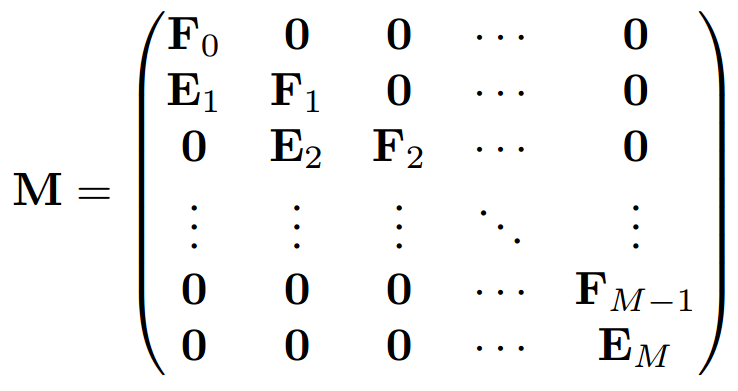
\includegraphics[width=3.0in]{ch5_3.png} 
    \caption{最终$\bm M$形式}
    \label{fig3} % 这里设置标签
\end{figure}
其中$\bm F_0,\bm E_M\in \mathbb{R}^{3\times 6},\bm E_i,\bm F_i\in \mathbb{R}^{6\times 6},\forall i\in [1,M-1]$,$M$为pieces个数。

最后按照上述推导依次完成代码中始末状态约束和每个piece的中间状态约束,代码附录A所示,运行结果如图\ref{fig4}所示
\begin{figure}[H]
    \centering
    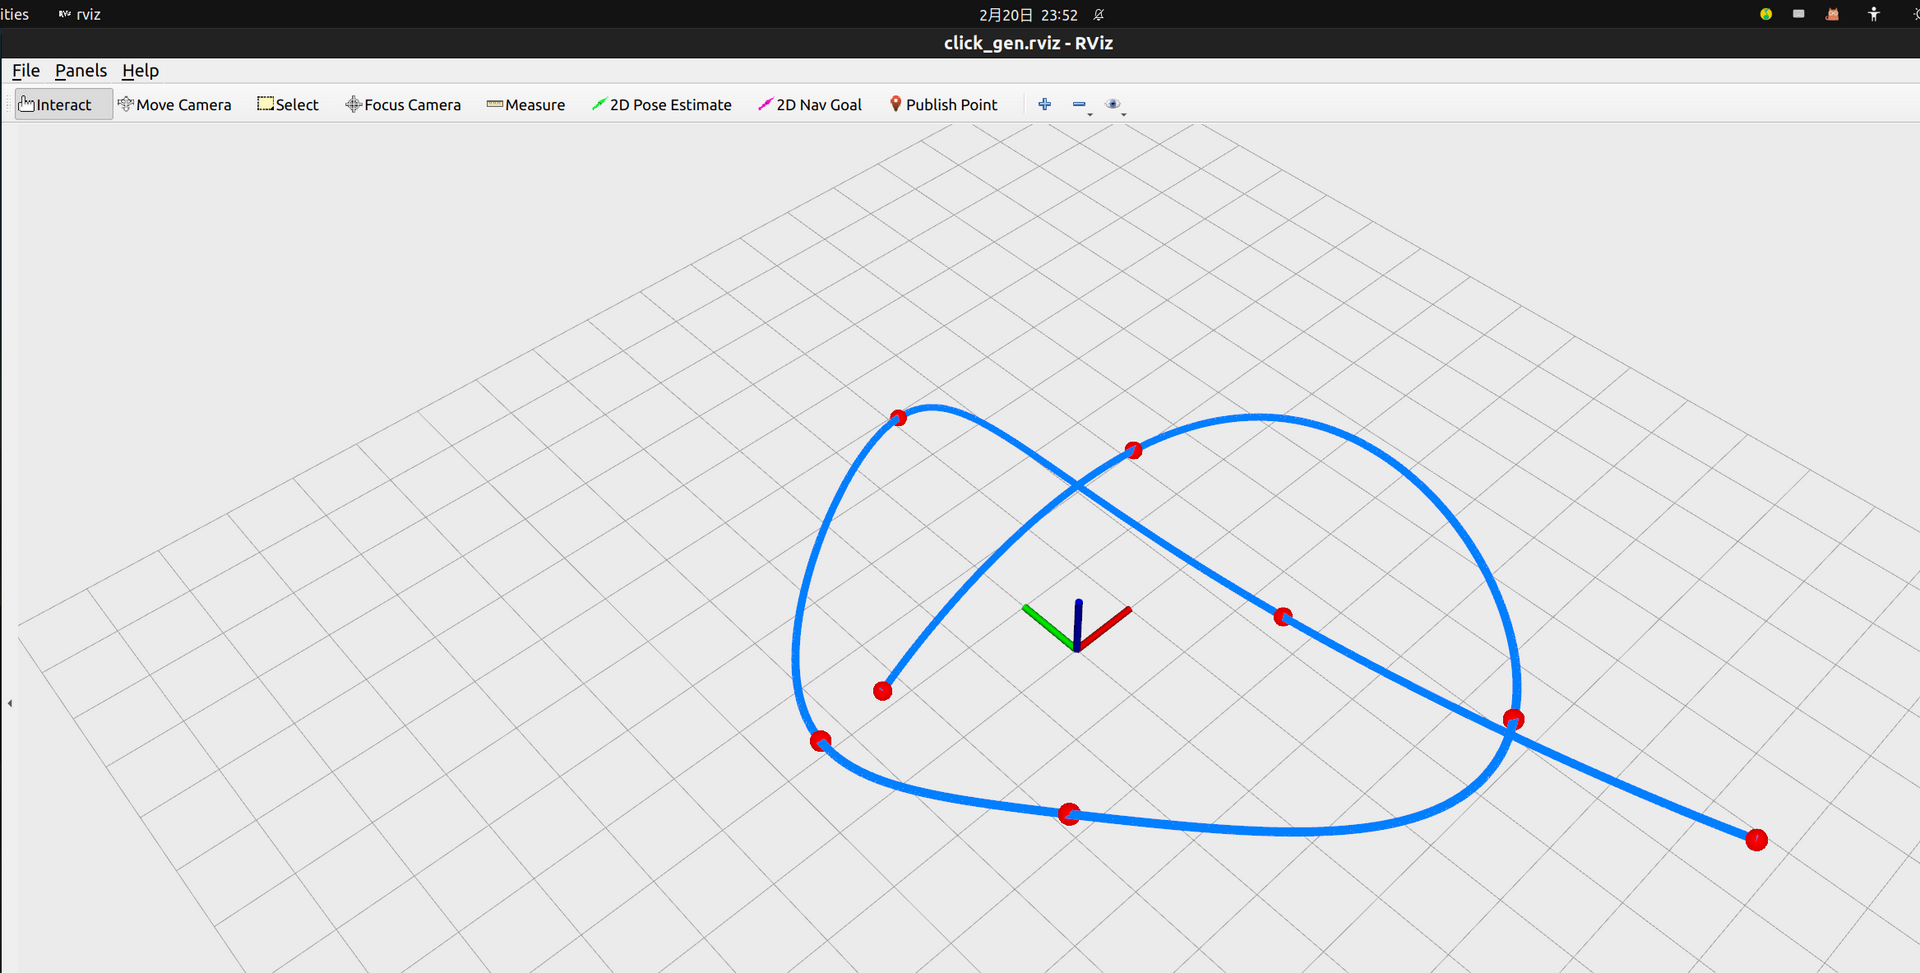
\includegraphics[width=3.0in]{ch5_4.png} 
    \caption{运行结果}
    \label{fig4} % 这里设置标签
\end{figure}

%在使用\ref{}命令之前,需要至少编译两次LaTeX文档。这是因为在第一次编译时,LaTeX会记录下各个标签所对应的编号,在第二次编译时才能正确替换引用。
\begin{thebibliography}{99}  
    \bibitem{ref1}Wang et al., Geometrically Constrained Trajectory Optimization for Multicopters, TRO 2022.
\end{thebibliography}


\clearpage 
\onecolumn
\appendix
\section{Appendix A}

% \begin{@twocolumnfalse}
    \begin{lstlisting}[language=C++, caption=click\_gen.cpp/minimumJerkTrajGen()]
        void minimumJerkTrajGen(
            // Inputs:
            const int pieceNum,
            const Eigen::Vector3d &initialPos,
            const Eigen::Vector3d &initialVel,
            const Eigen::Vector3d &initialAcc,
            const Eigen::Vector3d &terminalPos,
            const Eigen::Vector3d &terminalVel,
            const Eigen::Vector3d &terminalAcc,
            const Eigen::Matrix3Xd &intermediatePositions,
            const Eigen::VectorXd &timeAllocationVector,
            // Outputs:
            Eigen::MatrixX3d &coefficientMatrix)
        {
            // coefficientMatrix is a matrix with 6*piece num rows and 3 columes
            // As for a polynomial c0+c1*t+c2*t^2+c3*t^3+c4*t^4+c5*t^5,
            // each 6*3 sub-block of coefficientMatrix is
            // --              --
            // | c0_x c0_y c0_z |
            // | c1_x c1_y c1_z |
            // | c2_x c2_y c2_z |
            // | c3_x c3_y c3_z |
            // | c4_x c4_y c4_z |
            // | c5_x c5_y c5_z |
            // --              --
            // Please computed coefficientMatrix of the minimum-jerk trajectory
            // in this function
        
            // ------------------------ Put your solution below ------------------------
            //coefficientMatrix维度维度为(6*pieceNum, 3),之前已经给出,不用操作
            //起始和末状态的PVA约束分别是3行,加起来总共6行约束(s*2s)=(3*6),中间状态有(pieceNum-1)组约束(2s*2s)=(6*6),所以总约束仍为(2sM*2sM)=(6M*6M)
            Eigen::MatrixXd M = Eigen::MatrixXd::Zero(6*pieceNum, 6*pieceNum);
            Eigen::MatrixXd b = Eigen::MatrixXd::Zero(6*pieceNum, 3);
        
            //初始条件PVA约束
            Eigen::MatrixXd F_0(3, 6);
            F_0.setZero();
            F_0(0,0) = 1;
            F_0(1,1) = 1;
            F_0(2,2) = 2;
            M.block(0,0,3,6) = F_0;
            b.row(0) = initialPos.transpose();
            b.row(1) = initialVel.transpose();
            b.row(2) = initialAcc.transpose();
        
            //终止条件条件PVA约束
            Eigen::MatrixXd E_M(3, 6);
            double T_M = timeAllocationVector(pieceNum-1);
            double T_M_2 = T_M * T_M;
            double T_M_3 = T_M_2 * T_M;
            double T_M_4 = T_M_3 * T_M;
            double T_M_5 = T_M_4 * T_M;
            E_M <<  1,  T_M,    T_M_2,  T_M_3,      T_M_4,      T_M_5,
                    0,  1,      2*T_M,  3*T_M_2,    4*T_M_3,    5*T_M_4,
                    0,  0,      2,      6*T_M,      12*T_M_2,   20*T_M_3;
            M.block(6*pieceNum-3,6*(pieceNum-1),3,6) = E_M;
            b.row(6*pieceNum-3) = terminalPos.transpose();
            b.row(6*pieceNum-2) = terminalVel.transpose();
            b.row(6*pieceNum-1) = terminalAcc.transpose();
        
        
            //M共pieceNum-1组中间状态约束,前面F_0的3*6 PVA约束,后面E_M的3*6 PVA约束,
            //中间是pieceNum-1组中间状态约束,由waypoint,P,V,A,Jerk,Snap连续可导组成的E_i(6*6),F_i(6*6)约束
            for(int i = 1; i < pieceNum; ++i) {//这里使用的时间是左闭右开,中间点约束在左边点上,所以是从第[1]个而非第[0]个开始
                double T = timeAllocationVector(i-1);
                double T_2 = T * T;
                double T_3 = T_2 * T;
                double T_4 = T_3 * T;
                double T_5 = T_4 * T;
                Eigen::MatrixXd E_i(6, 6);
                Eigen::MatrixXd F_i(6, 6);
                E_i <<  1,  T,  T_2,    T_3,    T_4,    T_5,
                        1,  T,  T_2,    T_3,    T_4,    T_5,
                        0,  1,  2*T,    3*T_2,  4*T_3,  5*T_4,
                        0,  0,  2,      6*T,    12*T_2, 20*T_3,
                        0,  0,  0,      6,      24*T,   60*T_2,
                        0,  0,  0,      0,      24,     120*T;
                M.block(6*i-3, 6*(i-1), 6, 6) = E_i;
        
                F_i.setZero();
                F_i(1,0) = -1;
                F_i(2,1) = -1;
                F_i(3,2) = -2;
                F_i(4,3) = -6;
                F_i(5,4) = -24;
                M.block(6*i-3, 6*i, 6, 6) = F_i;
        
                Eigen::Vector3d D_i_transpose = intermediatePositions.block(0,i-1,3,1);
                b.block(6*i-3, 0, 1, 3) << D_i_transpose(0), D_i_transpose(1), D_i_transpose(2);
        
            }
        
            clock_t time_stt = clock();
            // 使用PartialPivLU进行分解
        //    Eigen::PartialPivLU<Eigen::MatrixXd> lu(M);
            // Mc = b 解为c
            std::cout << "use lu" <<std::endl;
            coefficientMatrix = M.lu().solve(b);
        
        /*    // Solve Mc = b, using QR solver
            for (int i = 0; i < 3; i++)
            {
                coefficientMatrix.col(i) = M.colPivHouseholderQr().solve(b.col(i));
        //         coefficientMatrix.col(i) = M.lu().solve(b.col(i));
            }
            coefficientMatrix = M.inverse() * b;*/
        
            // std::cout << "C is " << coefficientMatrix << std::endl;
            std::cout << "Time cost = " << 1000 * (clock() - time_stt) / (double)CLOCKS_PER_SEC << "ms" << std::endl;
        
            // ------------------------ Put your solution above ------------------------
        }
\end{lstlisting}
% \end{@twocolumnfalse}


\end{document}